\documentclass[16pt]{extarticle} 

\usepackage[margin=0.6in]{geometry} 
\usepackage{tikz,lipsum,lmodern} 
\usepackage[most]{tcolorbox} 
\usepackage[default]{lato} 
\usepackage[T1]{fontenc} 
\usepackage{tikz} 
\usepackage{dashrule} 
\usepackage{comment} 
\usepackage{eso-pic} 
\usepackage{ifthen} 
\usepackage{changepage} 
\usepackage{xcolor} 
\tcbuselibrary{listings,breakable} 

\definecolor{customBlack}{RGB}{46,50,48} 
\definecolor{buildBlue}{RGB}{198,214,230} 
\definecolor{codeBlue}{RGB}{211,237,237} 
\definecolor{businessBlue}{RGB}{156,202,202} 
\definecolor{lineBlue}{RGB}{0,89,89} 
\definecolor{textGrey}{RGB}{84,84,84} 
\definecolor{nameGrey}{RGB}{217,217,217} 
\definecolor{wholeBlue}{RGB}{188, 217, 223} 

\color{textGrey} 
\renewcommand{\baselinestretch}{1.3} 
\thispagestyle{empty} 

\begin{document}

\AddToShipoutPicture{ \checkoddpage 
    \ifoddpage \put(0,0){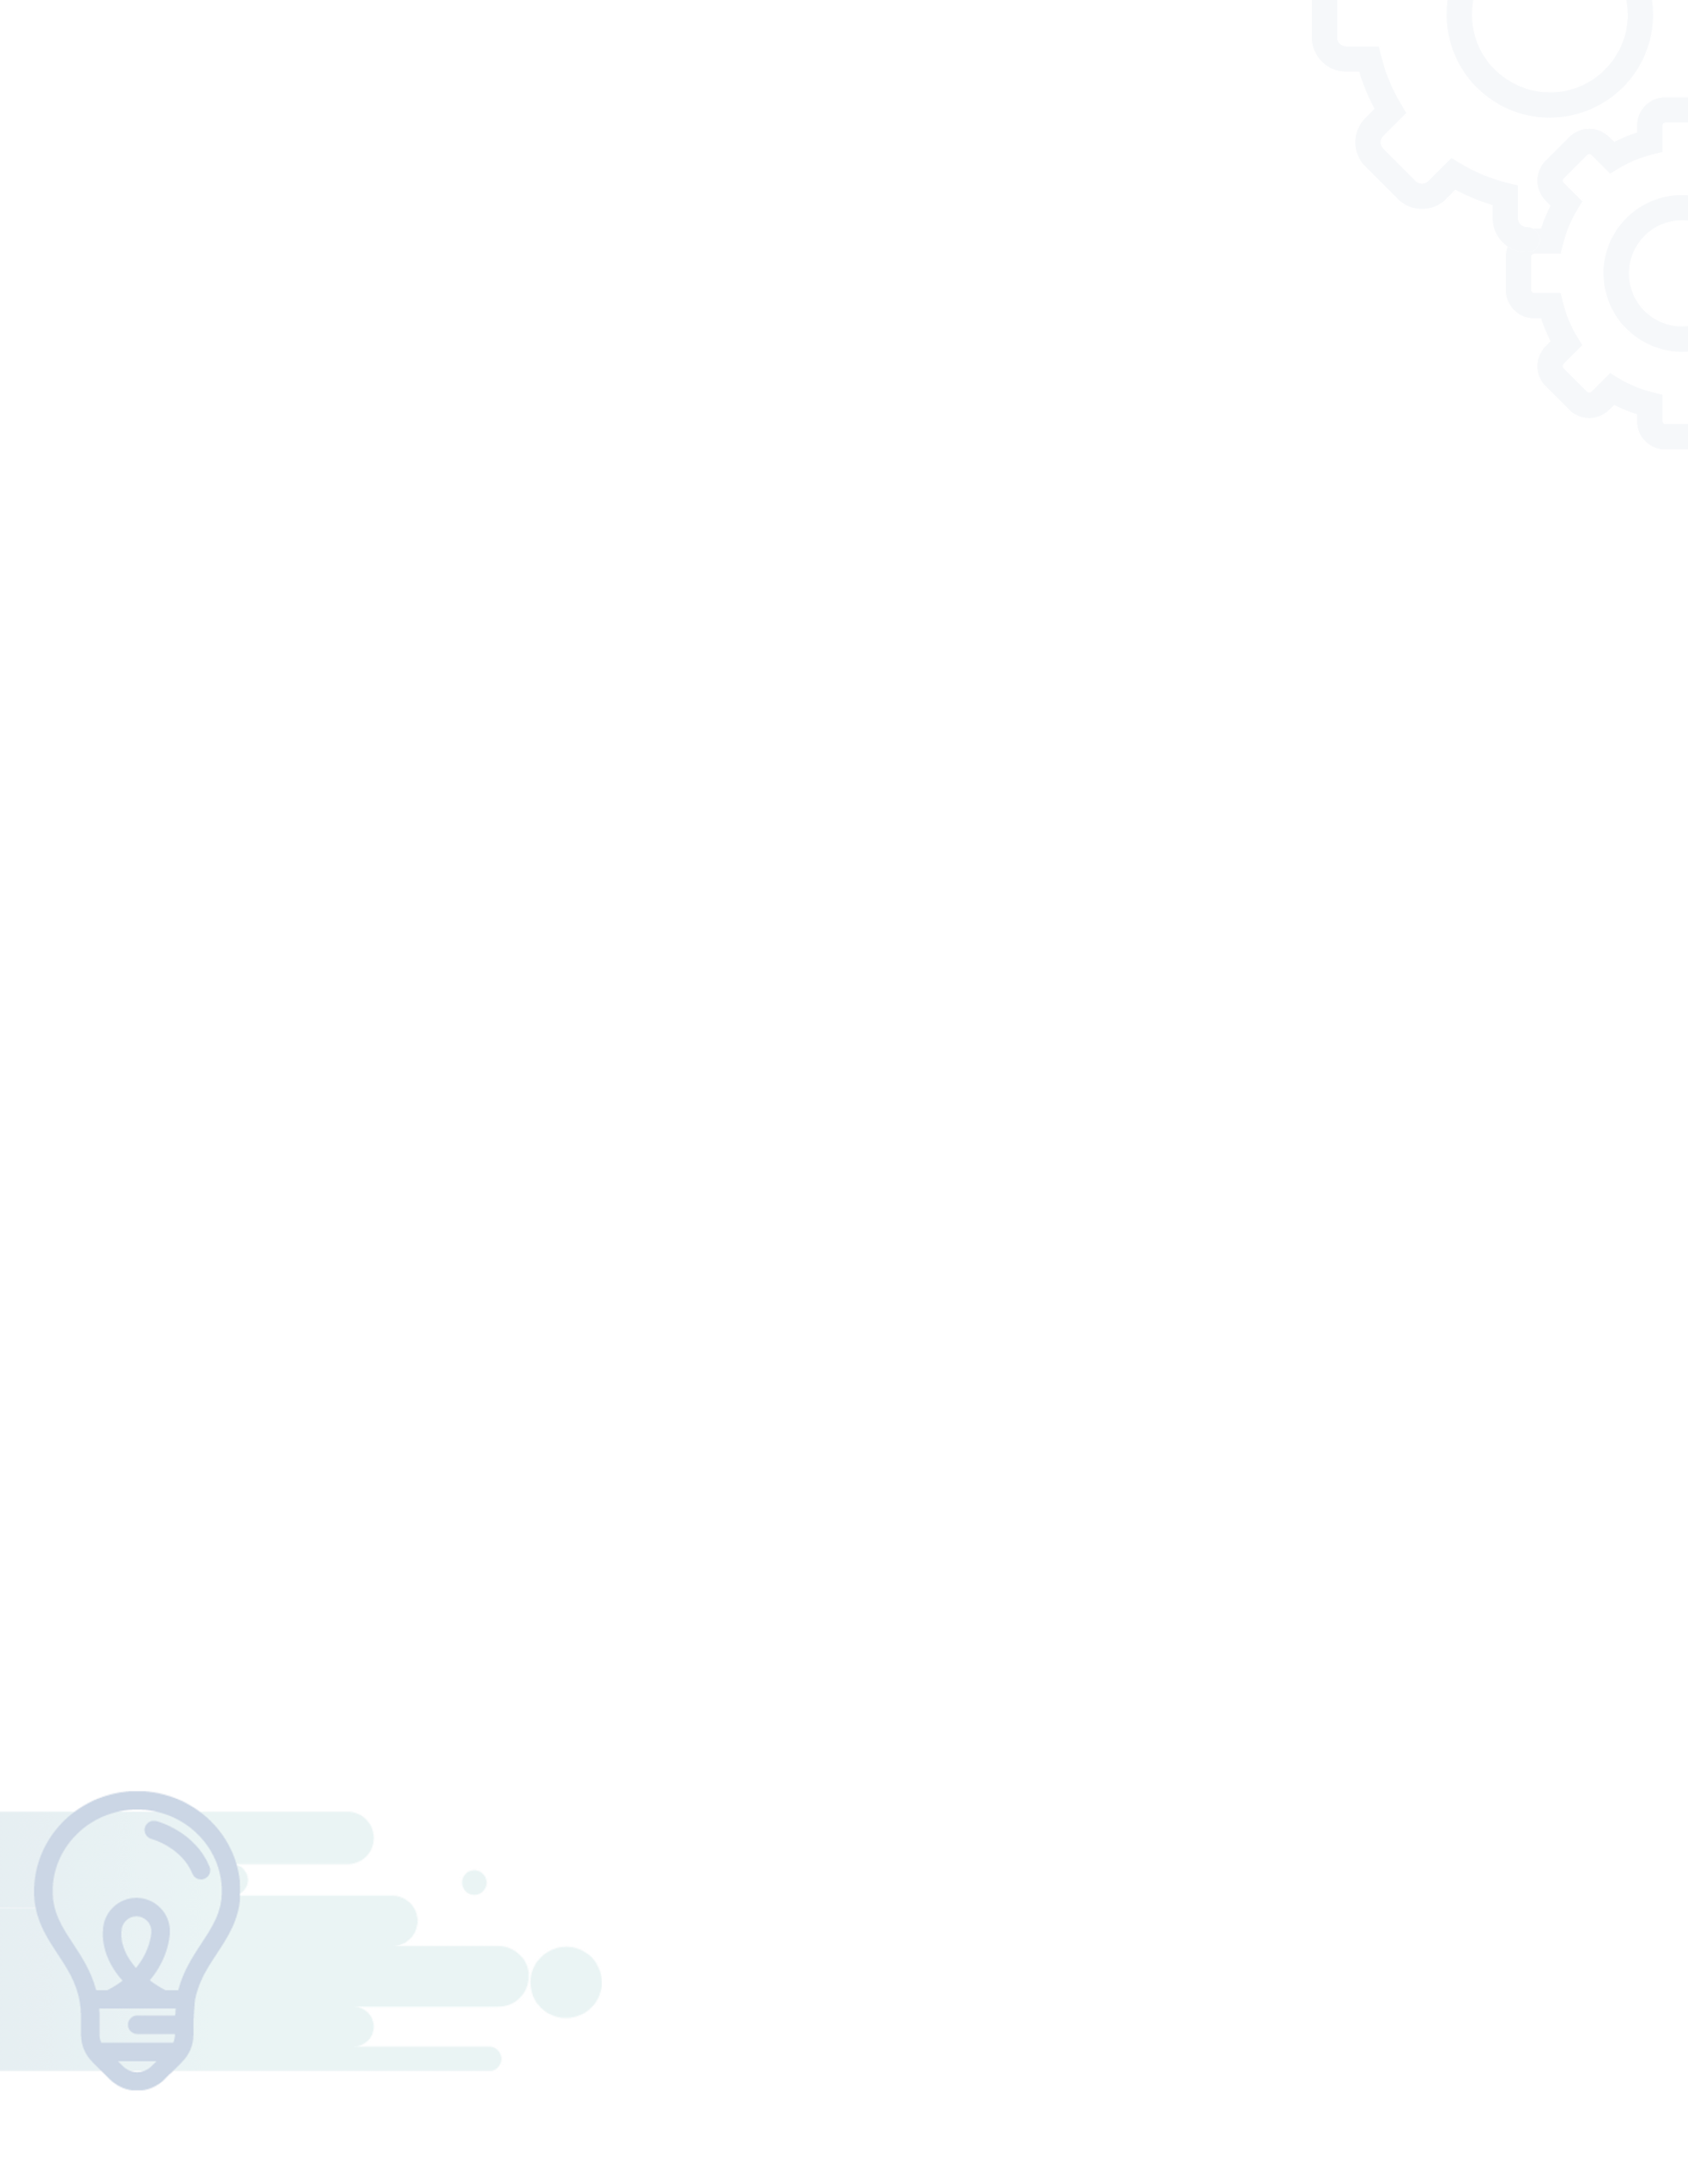
\includegraphics[width=\paperwidth]{../figs/oddPage2.png}} 
     \else     \put(0,0){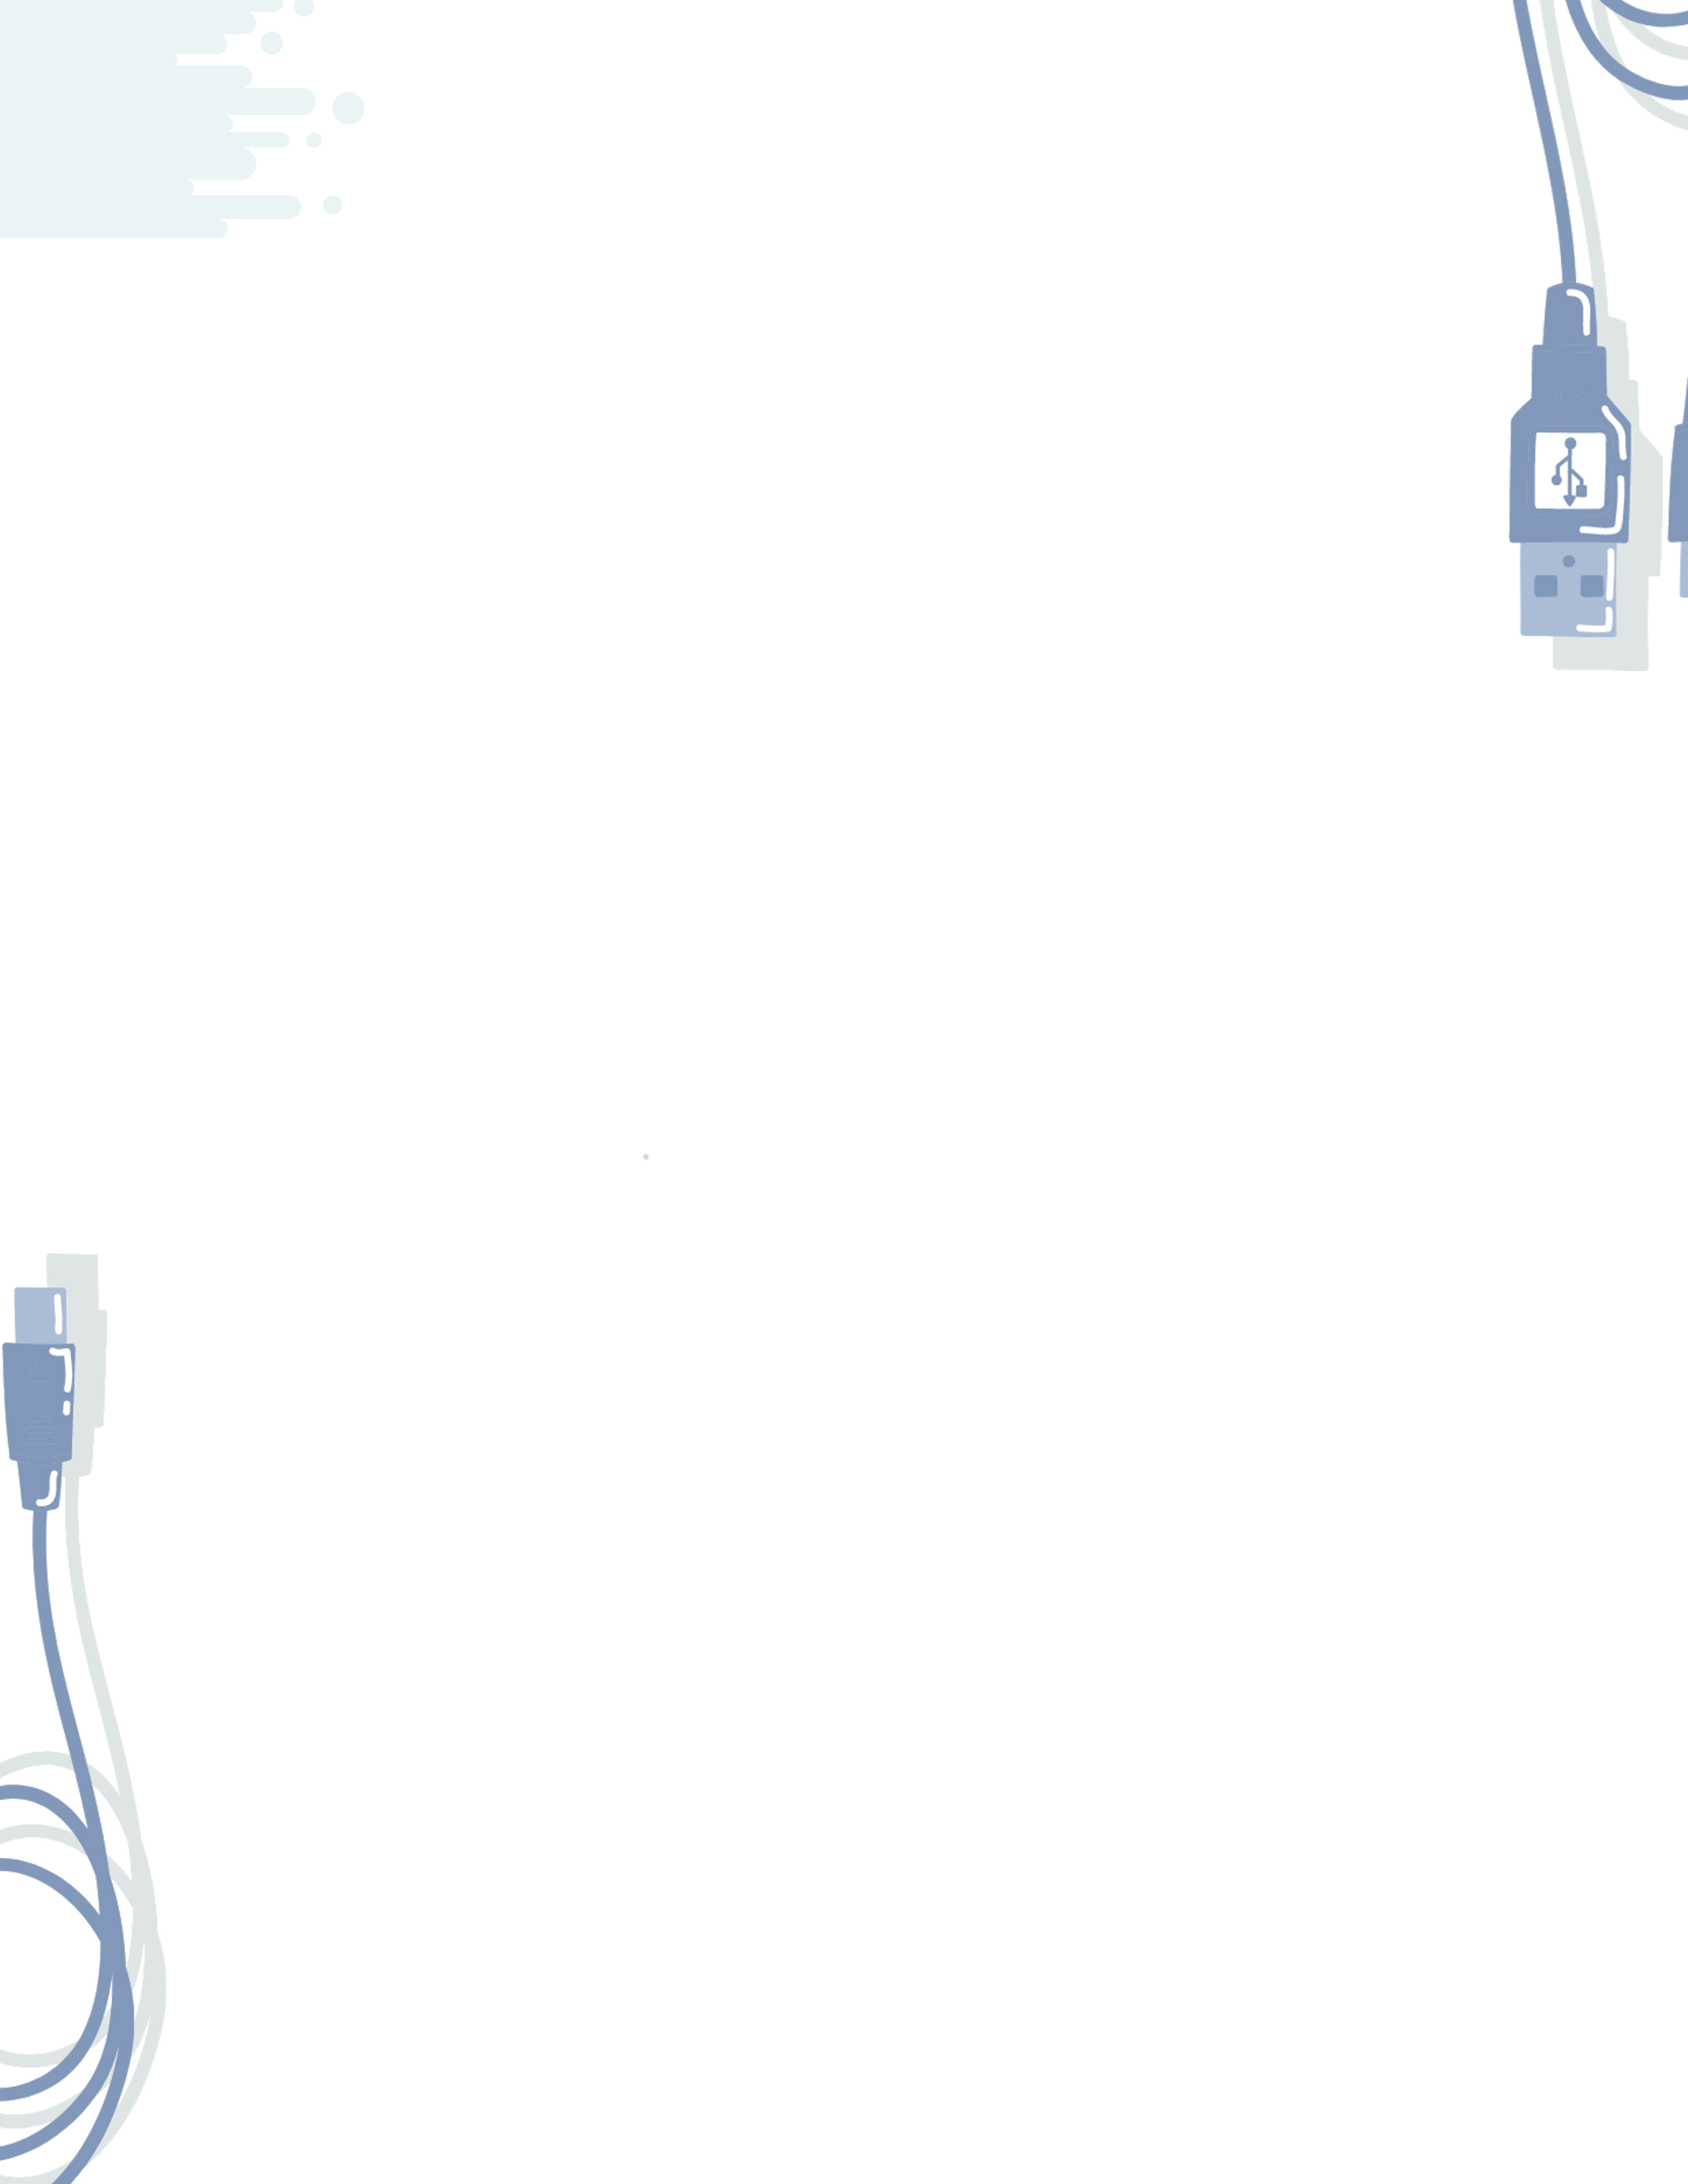
\includegraphics[width=\paperwidth]{../figs/evenPage.png}} 
\fi }

\begin{tcolorbox}[colback=customBlack,colframe=white!,coltext=white,sidebyside, lower separated=false, after skip=20pt plus 2pt]  
    {\Huge January 9, 2021}   \tcblower  \begingroup      
           \fontsize{11.9pt}{10pt}\selectfont     
           \textcolor{nameGrey}{ATTENDEES: Ellie, Marcus, Maya, Audrey C., Karla, Bonnie, Abby G., Abby B., Liza, Hannah, Audrey W., Sophia, Amelia, Alyssa, Karina}  
    \endgroup 
\end{tcolorbox}

{\Large \textbf{FOCUS }} \textcolor{lineBlue}{\hdashrule[0.5ex]{16.1cm}{0.5mm}{2mm 1.5pt}}
\begin{tcolorbox}[colback=wholeBlue,colframe=white!,coltext=textGrey]  
    \textit{\textbf{Entire Team: }}Group discussion about general engineering notebook layout Sub-team + individual portfolio writing
\end{tcolorbox}

{\Large \textbf{SUMMARY }} \textcolor{lineBlue}{\hdashrule[0.5ex]{15.2cm}{0.5mm}{2mm 1.5pt}}
\begin{tcolorbox}[colback=wholeBlue,colframe=white!,coltext=textGrey]  
    \textit{\textbf{Entire Team: }}At the start of the meeting, the team gathered to discuss components of our engineering notebook. First, we presented the different layout options created by our business team to the rest of our team members.  Different layout options included separating entries by subteam and sections labeled focus and challenges. Following, we separated into different breakout rooms to discuss our preffered layout. We also choose the cover for our engineering notebook. Following notebook discussion, we moved onto individual and subteam writing for the engineering portfolio. 
\end{tcolorbox}

{\Large \textbf{CHALLENGES }} \textcolor{lineBlue}{\hdashrule[0.5ex]{14.7cm}{0.5mm}{2mm 1.5pt}}
\begin{tcolorbox}[colback=wholeBlue,colframe=white!,coltext=textGrey]  
    \textit{\textbf{Entire Team: }}I think overall, the decisions from various breakout rooms were in unison. We were all able to come to an agreement on one of our layout options. 
\end{tcolorbox}

{\Large \textbf{NEXT STEPS }} \textcolor{lineBlue}{\hdashrule[0.5ex]{15cm}{0.5mm}{2mm 1.5pt}}
\begin{tcolorbox}[colback=wholeBlue,colframe=white!,coltext=textGrey]  
    \textit{\textbf{Entire Team: }}In terms of next steps, there is a lot of porfolio writing that needs to be  done. I think we did a good job of brainstorming topics we want to discuss within our different subteams. 
\end{tcolorbox}

\end{document}
